\documentclass{standalone}
\usepackage{tikz}
\begin{document}
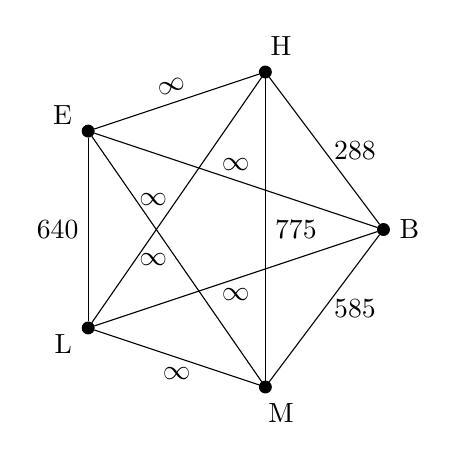
\begin{tikzpicture}
      \tikzset{enclosed/.style={draw, circle, inner sep=0pt, minimum size=.15cm, fill=black}}

      \node[enclosed, label={left, yshift=.2cm: E}] (E) at (0.75,3.25) {};
      \node[enclosed, label={above, xshift=.2cm: H}] (H) at (3,4) {};
      \node[enclosed, label={right, yshift=0cm: B}] (B) at (4.5,2) {};
      \node[enclosed, label={below, xshift=.2cm: M}] (M) at (3,0) {};
      \node[enclosed, label={left, yshift=-.2cm: L}] (L) at (0.75,0.75) {};

      \draw (E) -- (H) node[midway, sloped, above] (edge1) { $\infty$};
      \draw (H) -- (B) node[midway, right] (edge2) {288};
      \draw (B) -- (M) node[midway, right] (edge3) {585};
      \draw (L) -- (M) node[midway, below] (edge4) {$\infty$};
      \draw (E) -- (L) node[midway, left] (edge5) {640};
      \draw (E) -- (B) node[midway, above] (edge6) {$\infty$};
      \draw (E) -- (M) node[midway, left] (edge7) {$\infty$};
      \draw (L) -- (H) node[midway, left] (edge8) {$\infty$};
      \draw (L) -- (B) node[midway, below] (edge9) {$\infty$};
      \draw (H) -- (M) node[midway, right] (edge10) {775};
\end{tikzpicture}
\end{document}
